\documentclass[12pt,a4paper]{report}

\usepackage{mathptmx}
\usepackage{graphicx}
\usepackage{amsmath}
\usepackage{amssymb}
\usepackage{amsthm}
\usepackage{url}
\usepackage{hyperref}
\usepackage{setspace}
\usepackage{geometry}
\usepackage{titlesec}
\usepackage{tabularx}
\usepackage{longtable}
\usepackage{float}
\usepackage{xcolor}
\usepackage{algorithm}
\usepackage{algpseudocode}
\usepackage{caption}
\usepackage{chngcntr}
\usepackage{fancyhdr}
\usepackage{ragged2e}
\usepackage{etoolbox}
\usepackage{datetime}
\usepackage[backend=bibtex,style=ieee,sorting=none]{biblatex}
\usepackage{tikz}
\usetikzlibrary{shapes.geometric, arrows.meta, positioning, fit, backgrounds, shadows.blur}
\usepackage{eso-pic}
\usepackage{listings}
\lstdefinestyle{pythonstyle}{
  language=Python,
  basicstyle=\small\ttfamily,
  keywordstyle=\bfseries\color[RGB]{0,0,180},
  stringstyle=\color[RGB]{163,21,21},
  commentstyle=\itshape\color[RGB]{60,120,60},
  numberstyle=\tiny\color[RGB]{120,120,120},
  numbers=left,
  numbersep=8pt,
  stepnumber=1,
  breaklines=true,
  breakatwhitespace=false,
  columns=flexible,
  keepspaces=true,
  showstringspaces=false,
  frame=single,
  framesep=4pt,
  rulecolor=\color[RGB]{180,180,180},
  backgroundcolor=\color[RGB]{248,248,252},
  xleftmargin=20pt,
  xrightmargin=0pt,
  tabsize=4,
  captionpos=t,
  aboveskip=8pt,
  belowskip=8pt,
}
\lstset{style=pythonstyle}

% Page geometry with extra bottom margin for footer
\geometry{a4paper, left=1in, right=1in, top=1in, bottom=1.2in}
\setlength{\headheight}{27.12pt}

% --- Page border on every page ---
\AddToShipoutPictureBG{%
  \begin{tikzpicture}[remember picture, overlay]
    \draw[line width=1.5pt]
      ([xshift=0.5in, yshift=-0.5in] current page.north west)
      rectangle
      ([xshift=-0.5in, yshift=0.5in] current page.south east);
  \end{tikzpicture}%
}

\hypersetup{
    colorlinks=true,
    citecolor=blue,
    linkcolor=blue,
    urlcolor=blue
}

\renewcommand{\algorithmicrequire}{\textbf{Input:}}
\renewcommand{\algorithmicensure}{\textbf{Output:}}
\renewcommand{\algorithmiccomment}[1]{\hfill{\small\textit{#1}}}

\titleformat{\chapter}[block]
  {\normalfont\bfseries\fontsize{14}{16}\selectfont}
  {\chaptername\ \thechapter}{1em}{}
\titlespacing*{\chapter}{0pt}{12pt}{12pt}

\titleformat{\section}
  {\normalfont\bfseries\fontsize{12}{14}\selectfont}
  {\thesection}{1em}{}
\titleformat{\subsection}
  {\normalfont\bfseries\fontsize{12}{14}\selectfont}
  {\thesubsection}{1em}{}
\titleformat{\subsubsection}
  {\normalfont\bfseries\fontsize{12}{14}\selectfont}
  {\thesubsubsection}{1em}{}

\setlength{\parindent}{0.5in}
\setlength{\parskip}{0pt}

\newdateformat{mydateformat}{\twodigit{\THEDAY}-\twodigit{\THEMONTH}-\THEYEAR}

\captionsetup{font={small,stretch=1},labelfont=bf}
\let\footnotelayout\singlespacing
\AtBeginEnvironment{quote}{\singlespacing}

\numberwithin{equation}{chapter}
\counterwithin{figure}{chapter}
\counterwithin{table}{chapter}
\counterwithin{algorithm}{chapter}

\fancypagestyle{romanstyle}{
  \fancyhf{}
  \fancyfoot[L]{\small Dept. of CSE (Data Science), BMSCE}
  \fancyfoot[C]{\small 2025--2026}
  \fancyfoot[R]{\small\roman{page}}
  \renewcommand{\headrulewidth}{0pt}
  \renewcommand{\footrulewidth}{0.4pt}
}

\fancypagestyle{mainstyle}{
  \fancyhf{}
  \fancyhead[L]{\small\textbf{Robust Tonic Sa Detection and FSM-Based Raga Grammar Validation}}
  \fancyfoot[L]{\small Dept. of CSE (Data Science), BMSCE}
  \fancyfoot[C]{\small 2025--2026}
  \fancyfoot[R]{\thepage}
  \renewcommand{\headrulewidth}{0.4pt}
  \renewcommand{\footrulewidth}{0.4pt}
}

% Redefine 'plain' for roman-numbered front matter pages
\newcommand{\setplainstyle}[1]{%
  \fancypagestyle{plain}{
    \fancyhf{}
    \fancyfoot[L]{\small Dept. of CSE (Data Science), BMSCE}
    \fancyfoot[C]{\small 2025--2026}
    \fancyfoot[R]{\small#1}
    \renewcommand{\headrulewidth}{0pt}
    \renewcommand{\footrulewidth}{0.4pt}
  }
}

% Roman front matter plain style
\fancypagestyle{plainroman}{
  \fancyhf{}
  \fancyfoot[L]{\small Dept. of CSE (Data Science), BMSCE}
  \fancyfoot[C]{\small 2025--2026}
  \fancyfoot[R]{\small\roman{page}}
  \renewcommand{\headrulewidth}{0pt}
  \renewcommand{\footrulewidth}{0.4pt}
}

% Redefine 'plain' (used on chapter opening pages) to match mainstyle footer
\fancypagestyle{plain}{
  \fancyhf{}
  \fancyfoot[L]{\small Dept. of CSE (Data Science), BMSCE}
  \fancyfoot[C]{\small 2025--2026}
  \fancyfoot[R]{\thepage}
  \renewcommand{\headrulewidth}{0pt}
  \renewcommand{\footrulewidth}{0.4pt}
}

\addbibresource{biblio.bib}

\begin{document}
\onehalfspacing

\begin{titlepage}
    \begin{center}
        \textsc{\Large \textbf{B.M.S. COLLEGE OF ENGINEERING}}\\[0.2cm]
        \textsc{\large \textbf{(Autonomous College under VTU)}}\\[0.2cm]
        \textsc{\large \textbf{Bull Temple Road, Basavangudi, Bangalore - 560019}}\\[0.5cm]

        
\includegraphics[scale=0.75]{logo.png}\\[0.2cm]
        \textit{A thesis on}\\[0.2cm]
        \textsc{\textbf{Robust Tonic Sa Detection and FSM-Based Raga Grammar Validation for Carnatic Practice}}\\[0.2cm]
        \textit{in fulfillment of the requirements for the award of degree}\\[0.2cm]

        \textbf{BACHELOR OF ENGINEERING}\\[0.15cm]
        \textit{in}\\[0.2cm]
        \textbf{Computer Science \& Engineering (Data Science)}\\[0.2cm]

        \textit{by}\\[0.2cm]
        \textbf{G Shreekar (1BM23CD018)}\\[0.2cm]
        \textbf{H Sampreeth Bhat (1BM23CD020)}\\[0.2cm]
        \textbf{R V Abhishek (1BM23CD047)}\\[0.85cm]

        \textbf{Under the Guidance of}\\[0.25cm]
        \textbf{Dr. Shambhavi B R}\\[0.15cm]
        Assistant Professor\\[0.55cm]
        \textbf{Department of CSE (Data Science)}\\
        \textbf{B.M.S. College of Engineering}\\[0.3cm]

        \textbf{AY 2025--2026}
    \end{center}
\end{titlepage}

\pagenumbering{roman}
\pagestyle{romanstyle}

\chapter*{Certificate}
\thispagestyle{romanstyle}
\addcontentsline{toc}{chapter}{Certificate}
\begin{center}
    \textsc{\Large \textbf{B.M.S. COLLEGE OF ENGINEERING}}\\[0.1cm]
    \textsc{\large \textbf{(Autonomous College under VTU)}}\\[0.1cm]
    \textsc{\large \textbf{Bull Temple Road, Basavangudi, Bangalore - 560019}}\\[0.4cm]

    
\includegraphics[scale=0.4]{logo.png}\\[0.1cm]
    \textbf{Department of Computer Science and Engineering (Data Science)}\\[0.1cm]
    \textbf{\Large \underline{CERTIFICATE}}\\[0.1cm]
\end{center}

\noindent
This is to certify that the project entitled ``\textbf{Robust Tonic Sa Detection and FSM-Based Raga Grammar Validation for Carnatic Practice}'' is a bona fide work carried out by the following students for the course Project Work -- Phase 2 (Course Code: \textbf{23DS7PWPP2}). It is certified that all corrections and suggestions indicated during the internal assessments have been incorporated in the final thesis submitted to the departmental library. The project thesis has been approved as it meets the academic requirements prescribed for the Bachelor of Engineering degree in respect of project work.

\begin{center}
    \textbf{\underline{Candidate details}}
\end{center}

\begin{center}
\begin{tabularx}{\textwidth}{|c|X|c|}
    \hline
    \textbf{SL. NO.} & \textbf{Student Name} & \textbf{USN} \\
    \hline
    1 & G Shreekar & 1BM23CD018 \\
    \hline
    2 & H Sampreeth Bhat & 1BM23CD020 \\
    \hline
    3 & R V Abhishek & 1BM23CD047 \\
    \hline
\end{tabularx}
\end{center}

\vspace{1cm}

\begin{center}
\begin{tabular*}{\textwidth}{@{\extracolsep{\fill}} l c r}
\textbf{Dr. Kalyan N} & \textbf{Dr. Shambhavi B R} & \textbf{Dr. Bheemsha Arya} \\
Assistant Professor & Professor \& HOD & Principal \\
\end{tabular*}
\end{center}

\vspace{0.2cm}
\noindent
\textbf{Examiners}\\[0.1cm]
\textbf{Name of Examiner} \hfill \textbf{Signature of the examiner} \\[0.1cm]
\textbf{1.} \hfill \rule{5cm}{0.4pt} \\[0.1cm]
\textbf{2.} \hfill \rule{5cm}{0.4pt} \\

\newpage
\chapter*{Declaration}
\thispagestyle{romanstyle}
\addcontentsline{toc}{chapter}{Declaration}
\begin{center}
    \textsc{\Large \textbf{B.M.S. COLLEGE OF ENGINEERING}}\\[0.2cm]
    \textsc{\large \textbf{(Autonomous College under VTU)}}\\[0.2cm]
    \textsc{\large \textbf{Bull Temple Road, Basavangudi, Bangalore - 560019}}\\[0.5cm]
    
\includegraphics[width=0.2\textwidth]{logo.png}\\[0.2cm]
\end{center}

\begin{center}
    \textbf{\Large \underline{DECLARATION}}
\end{center}

\noindent
We hereby declare that the project thesis entitled ``\textbf{Robust Tonic Sa Detection and FSM-Based Raga Grammar Validation for Carnatic Practice}'' is a bona fide work and has been carried out by us under the guidance of \textbf{Dr. Shambhavi B R}, Assistant Professor, Department of Computer Science and Engineering (Data Science), B.M.S. College of Engineering, Bengaluru, in partial fulfillment of the requirements of the degree of Bachelor of Engineering in Computer Science \& Engineering (Data Science) of Visvesvaraya Technological University, Belagavi.
We further declare that, to the best of our knowledge and belief, this thesis has not been submitted either in part or in full to any other university or college.

\vspace{0.3cm}
\begin{center}
    \textbf{\underline{Candidate details}}
\end{center}

\begin{center}
\begin{tabularx}{\textwidth}{|c|X|c|c|}
    \hline
    \textbf{SL. NO.} & \textbf{Student Name} & \textbf{USN} & \textbf{Student Signature} \\
    \hline
    1 & G Shreekar & 1BM23CD018 & \\
    \hline
    2 & H Sampreeth Bhat & 1BM23CD020 & \\
    \hline
    3 & R V Abhishek & 1BM23CD047 & \\
    \hline
\end{tabularx}
\end{center}

\vspace{0.9cm}
\begin{flushleft}
    Date: \mydateformat\today
\end{flushleft}

\newpage
\chapter*{Acknowledgments}
\thispagestyle{romanstyle}
\addcontentsline{toc}{chapter}{Acknowledgments}
\noindent
We express our sincere gratitude to the management and faculty of B.M.S. College of Engineering for providing the resources and academic environment to complete this capstone project. We thank \textbf{Dr. Shambhavi B R} for her guidance, technical inputs, and continuous support. We also thank the Department of CSE (Data Science) for their feedback during the internal reviews and for enabling the infrastructure used for experiments and demonstrations.

\vspace{1.2cm}
\begin{flushright}
G Shreekar (1BM23CD018)\\
H Sampreeth Bhat (1BM23CD020)\\
R V Abhishek (1BM23CD047)\\
\end{flushright}

\newpage
\chapter*{Abstract}
\thispagestyle{romanstyle}
\addcontentsline{toc}{chapter}{Abstract}
Carnatic music is one of the world's most precisely codified melodic systems, in which every note is defined as an exact frequency ratio relative to a performer-chosen tonic Sa, and raga identity is enforced by strict ascending (arohana) and descending (avarohana) grammar rules. Student practice traditionally relies on a teacher who listens for microtonal deviations and grammar violations in real time---a process that is subjective, time-intensive, and difficult to replicate at scale during unsupervised practice.

This thesis presents a real-time Carnatic music practice assistant that addresses three core problems simultaneously: robust tonic Sa detection, microtonal swara quantization, and rule-based raga grammar validation with immediate feedback. The tonic detection engine employs a Carnatic harmonic product spectrum (HPS) ensemble that exploits the tambura drone's characteristic Sa--Pa frequency pair to score candidate frequencies. A coarse scan at 0.5\,Hz resolution identifies strong candidates, followed by a fine scan at 0.1\,Hz resolution within a narrow window, achieving sub-1\% error on benchmark recordings. A cross-validation step compares the Carnatic HPS result against an independent standard HPS estimate and selects secondary candidates when the primary estimate is a false positive caused by a dominant sung note.

Once Sa is locked, all twelve Carnatic swaras are computed from exact just-intonation ratios. Incoming frames are processed through a pYIN pitch tracker restricted to a tonic-relative band, passed through median and exponential moving average (EMA) filters, and matched to the nearest swara within a $\pm$35 cent tolerance window. A confidence score proportional to proximity drives downstream decisions.

The raga grammar validator is a multi-phase finite state machine. Phase 1 performs O(1) membership checks using direction-aware varja (forbidden note) sets. Phase 2 tracks octave-aware pairwise direction to distinguish ascending from descending motion across octave boundaries. Phase 3 derives vakra (zigzag) forbidden skip pairs automatically from the raga scale and detects illegal jumps using a rolling phrase buffer. Phase 4 recognizes characteristic prayoga (signature phrase) completions and generates positive reinforcement. Phase 5 produces multi-language (English, Kannada, Tamil, Telugu), context-aware teacher-like feedback messages. A time-based alert debouncer (950\,ms trigger, 600\,ms clear) suppresses false positives during melodic glides.

The system processes audio at approximately 35\,ms per frame and achieves end-to-end latency of about 70\,ms including the 1-second bootstrap. It reliably detects all 12 swaras within $\pm$35 cents and rejects silence, unvoiced frames, and glide transients using a four-layer gate. Tonic detection error on benchmark recordings averages 1.45\,\% (under 2\,Hz). A FastAPI server with WebSocket streaming delivers live feedback to a browser dashboard.

\noindent\textbf{Keywords:} Carnatic music, tonic detection, swara quantization, raga grammar, finite state machine, real-time audio processing, pitch tracking, music information retrieval, explainable feedback

\newpage
\tableofcontents
\newpage
\listoftables
\newpage
\listoffigures
\newpage
\chapter*{List of Abbreviations}
\thispagestyle{romanstyle}
\addcontentsline{toc}{chapter}{List of Abbreviations}
\begin{tabularx}{\textwidth}{|l|X|}
\hline
\textbf{Abbreviation} & \textbf{Meaning} \\
\hline
F0 & Fundamental frequency \\
HPS & Harmonic product spectrum \\
FSM & Finite state machine \\
STFT & Short-time Fourier transform \\
YIN & Autocorrelation-based pitch detector (Yet another INtonation method) \\
pYIN & Probabilistic YIN pitch tracker \\
MPM & McLeod Pitch Method \\
EMA & Exponential moving average \\
RMS & Root mean square \\
ASIC & Application-Specific Integrated Circuit \\
CNN & Convolutional neural network \\
DCNN & Deep convolutional neural network \\
DNN & Deep neural network \\
LSTM & Long short-term memory network \\
TDNN & Time-delay neural network \\
XAI & Explainable artificial intelligence \\
NLP & Natural language processing \\
MFCC & Mel-frequency cepstral coefficient \\
MIR & Music information retrieval \\
PCM & Pulse-code modulation \\
SDG & Sustainable Development Goal \\
API & Application programming interface \\
UI & User interface \\
WebSocket & Full-duplex browser communication protocol \\
Sa & Shadja -- the tonic note in Carnatic music \\
Sr & Sample rate \\
\hline
\end{tabularx}

\newpage
\pagenumbering{arabic}
\setcounter{page}{1}
\pagestyle{mainstyle}

\chapter{Introduction}
\section{Background}
Carnatic music is a highly structured melodic system where every performance is anchored to a performer-specific tonic Sa. All other swaras are defined as ratios relative to the tonic, and raga identity is governed by strict grammar rules in ascending and descending motion. For student practice, feedback is typically provided by a teacher who listens for microtonal deviations and forbidden notes. This process is time-consuming and subjective, and it becomes difficult to scale for continuous solo practice. A real-time assistant that can lock the tonic, track pitch accurately, and validate raga grammar can significantly improve the quality and consistency of training.

Modern raga recognition systems focus on classification using audio features and deep learning models, but they often ignore microtonal deviations and do not provide immediate, actionable feedback. Furthermore, tonic detection is typically treated as a preprocessing step rather than a first-class problem. In this project, tonic detection and grammar validation are central, enabling both accurate swara mapping and rule-based feedback. The result is an automated music teacher that assists students in maintaining pitch fidelity and raga correctness during live singing.

\section{Objectives}
\begin{enumerate}
    \item Detect the tonic Sa from short bootstrap audio using a robust Carnatic HPS ensemble.
    \item Map incoming vocal pitch to Carnatic swaras using exact ratios and a strict cents tolerance window.
    \item Validate swaras against raga grammar rules using a finite state machine with direction awareness.
    \item Provide real-time feedback with low latency and clear confidence scoring.
    \item Integrate the full pipeline into a live dashboard for practice and visualization.
\end{enumerate}

\section{Problem Statement}
Existing raga recognition systems do not offer real-time microtonal feedback and rarely enforce grammar constraints at the note level. Pitch detectors tuned for Western scales often introduce octave errors and misclassifications when the tonic is not explicitly locked. As a result, students lack a consistent method to validate swaras and grammar during practice. The core problem addressed in this thesis is to design a low-latency system that detects tonic Sa reliably, maps pitch to swaras with microtonal precision, and validates each swara against raga grammar to provide immediate corrective feedback.

\section{Summary}
This chapter introduced the motivation for real-time Carnatic practice feedback, defined the objectives, and stated the core problem. Chapter 2 reviews related work in raga recognition, pitch tracking, and explainable models. Chapter 3 presents the system architecture and methodology. Chapter 4 details the implementation, while Chapter 5 reports results and performance. Chapter 6 concludes the thesis and outlines future extensions.

\chapter{Literature Review}

\section{Audio Preprocessing and CNN-Based Raga Recognition}
Hebbar and Jagtap \cite{hebbar2023comparison} conducted a systematic comparison of audio preprocessing techniques for raga classification using the CMD-40 dataset containing 480 songs across 40 ragas. By converting raw audio to Mel-spectrograms and training 2D CNNs, they achieved 98.1\% classification accuracy. Their work demonstrates that CNN-based feature learning outperforms hand-crafted features and that spectral representation is highly discriminative for raga signatures. However, the system operates entirely offline and does not address microtonal precision or real-time grammar enforcement, which this project remedies through 22-shruti quantization and FSM-based validation.

The IEEE Transactions on Multimedia study on deep learning-based classification \cite{ieee2022deep} extended this further by training deep convolutional neural networks (DCNNs) on high-resolution spectrograms, automatically extracting hierarchical features from nonlinear raga structures. While achieving strong offline accuracy, the framework does not produce feedback granular enough for student practice.

\section{Pitch Tracking for Carnatic Music}
Krishnaswamy \cite{krishnaswamy2018application} addressed the fundamental challenge of pitch tracking in South Indian classical music using short-time Fourier transforms (STFT). Since Carnatic music uses a relative tonic rather than fixed Western pitches, standard pitch detectors fail to capture the required nuances. Krishnaswamy's framework establishes reliable fundamental frequency (F0) extraction as an absolute prerequisite for subsequent microtonal mapping---a principle adopted directly in this project's tonic-first pipeline design.

Foundational pitch estimators such as YIN \cite{decheveigne2002yin} and pYIN \cite{mauch2014pyin} establish the robustness requirements for low-noise F0 tracking, while CREPE \cite{kim2018crepe} demonstrates that deep representations can also estimate pitch accurately in difficult acoustic conditions. For polyphonic melody extraction, Salamon and Gómez \cite{salamon2012melody} show how contour-based post-processing improves stability, and Bittner et al. \cite{bittner2017deepsalience} extend this idea with deep salience maps for polyphonic F0 estimation. These works collectively motivate the tonic-band restriction and temporal smoothing used in this thesis.

In broader music information retrieval, Tzanetakis and Cook \cite{tzanetakis2002genre} and Klapuri and Davy \cite{klapuri2006signal} demonstrate that robust audio understanding requires carefully designed signal-processing stages before higher-level classification. Their findings support the decision to keep tonic detection and swara quantization deterministic rather than delegating the entire pipeline to an opaque classifier.

The ISMIR 2020 work on melody extraction from polyphonic signals \cite{ismir2020melody} achieved real-time F0 tracking of lead melody against dense accompaniment using CNNs, demonstrating that low-latency melody isolation (under 50\,ms) is technically feasible. This project builds on that latency benchmark, using pYIN pitch tracking restricted to a tonic-relative band to achieve similar responsiveness without requiring a deep learning model.

The ICASSP 2019 work on singing voice separation \cite{icassp2019singing} demonstrated vocal pitch extraction via deep neural networks and adaptive pitch tracking with 30--40\,ms latency, confirming that the sub-50\,ms real-time constraint targeted in this project is achievable. The system combines vocal isolation with pitch estimation, a concept adapted here as tonic-band restriction that eliminates non-vocal frequency candidates before pitch estimation.

\section{Sequence Modeling and Grammar-Aware Recognition}
Peri \cite{peri2023applying} introduced a paradigm of treating raga recognition as a document classification problem using hierarchical attention networks trained on CMD and HMD datasets. By processing note sequences analogously to sentences in NLP, the system learns grammar patterns in arohana--avarohana transitions. This work directly motivates grammar-aware sequence validation and is extended in this project from passive classification to active real-time rule enforcement.

The broader sequence-modeling literature also supports the design choices in this thesis. Long short-term memory networks \cite{hochreiter1997lstm} provide a principled way to retain melodic context, and attention mechanisms \cite{vaswani2017attention} improve the selection of salient note transitions in long sequences. Although this thesis does not train a neural sequence model, its rolling phrase buffer and longest-suffix matching emulate the contextual memory that these models learn from data.

Optimization and regularization techniques from general deep learning literature remain relevant for comparing deterministic and learned systems. Adam \cite{kingma2015adam} is widely used to stabilize training, while residual learning \cite{he2016resnet} reduces degradation in deep models. These methods are not required in the rule-based validator, but they form the benchmark against which the thesis positions a simpler and more explainable approach.

Natesan and Beigi \cite{natesan2020carnatic} combined TDNNs, LSTMs, and attention mechanisms tested on 676 songs spanning 172 ragas, achieving 95.31\% classification accuracy. The temporal modeling explicitly traces arohana and avarohana patterns, and the attention mechanism highlights critical melodic phrases. The present project adapts these insights into a finite state machine with direction-aware phrase tracking that operates without training data.

\section{Ensemble Learning and Feature Fusion}
The stacked ensemble learning study \cite{arxiv2022carnatic} demonstrated that aggregating multiple classifiers significantly reduces variance and bias compared to single-model approaches, and that multi-modal feature fusion (Mel-spectrograms, F0 contours, chroma features, 22-shruti quantization) improves robustness for overlapping raga signatures. This motivates the ensemble approach in tonic detection, where the Carnatic HPS result is cross-validated against a standard HPS estimate to resolve ambiguous cases.

\section{Explainable AI for Raga Identification}
The ISMIR 2023 study \cite{ismir2023explainable} applied XAI techniques to deep learning raga models to verify alignment with human expert understanding---specifically checking whether the model weighted gamakas (pitch oscillations) and anchor notes appropriately. For a pedagogical tool, conceptual explainability is critical: students must be able to trust and act on the feedback. This work directly motivates the transparent FSM design in this project, where every error is attributed to a specific rule and accompanied by an explanation of the raga's scale.

General interpretability methods also reinforce this design choice. Ribeiro et al. \cite{ribeiro2016why} show how local explanations can make classifier behavior actionable, Lundberg and Lee \cite{lundberg2017unified} provide a unified Shapley-value framework for feature attribution, and Grad-CAM \cite{selvaraju2017gradcam} demonstrates how visual explanations improve model debugging. These methods underline the pedagogical advantage of this thesis: instead of approximating an explanation after classification, the system encodes the explanation directly into the validation rule that fires.

\section{Phrase Analysis and Pitch Distribution Methods}
The IJCA 2015 study \cite{ijca2015phrase} explored raga recognition through statistical pitch distributions and phrase analysis, building probabilistic maps of arohana and avarohana note frequencies. This classical approach is an early precursor to the FSM phrase buffer used in this project, extended from passive recognition to active forbidden-skip detection and characteristic prayoga recognition.

The NCC 2022 study on raga space visualization \cite{ncc2022raga} applied t-SNE dimensionality reduction to map multi-raga datasets into a lower-dimensional space, demonstrating that microtonal shruti patterns form distinct clusters. This provides mathematical grounding for the 22-shruti quantization in this project, where continuous pitch frequencies are mapped to discrete shruti intervals and deviations in cents are computed and displayed to the student.

\section{Microtonal and Vector Space Modeling}
The Pattern Recognition Letters study \cite{prl2021vector} presented a vector space model based on 22-shruti quantization, mapping continuous pitch to discrete microtonal intervals. Accuracy improved from 88\% to 94\% when microtonal awareness was added. This work is one of the most critical foundations for this project; the apashruthi (microtonal deviation) detection engine adopts the same cent-based mapping and transforms it into a real-time diagnostic that quantifies how far a student's sung note deviates from the target swara.

The IEEE Signal Processing Letters study on self-extracting feature maps \cite{ieee2021self} demonstrated adaptive feature extraction that dynamically focuses on acoustically relevant signal components. This is relevant to the tonic detection engine, which uses median spectra and weighted harmonic scoring rather than rigid fixed transforms, allowing the detector to adapt to different vocal timbres and recording environments.

\section{Comparative Analysis and System Benchmarks}
The ICIDS 2021 comparative study \cite{ic2021comparative} systematically benchmarked AI classifiers for raga identification, documenting accuracy, computational efficiency, and processing latency. Their analysis confirms that lightweight models capable of sub-50\,ms classification are feasible and justifies the deterministic, rule-based architecture chosen in this project, which achieves 35\,ms per frame without any machine learning inference.

The JASI 2021 investigation \cite{jasi2021investigation} conducted a detailed acoustic analysis of raga-specific pitch distributions and swara combinations, highlighting the structural context required for reliable identification. The treatment of vivaadi swaras (forbidden notes) and 22-shruti scale patterns in that study directly informs the varja set definitions in the raga database used here.

\section{Limitations in Existing Systems}
Current raga systems share several key gaps relative to the requirements of a real-time practice assistant. First, they operate offline on complete recordings rather than on streaming frames, introducing latency incompatible with interactive practice. Second, tonic detection is typically a weak preprocessing step that fails when dominant sung notes or accompaniment obscures the tambura drone. Third, grammar validation at the note level---distinguishing allowed from forbidden swaras in the context of melodic direction---is absent in nearly all published systems. Fourth, feedback is not explainable: students receive a classification label but not an actionable correction. This project directly addresses all four gaps through its tonic-first ensemble design, direction-aware FSM, and teacher-modeled feedback generation.

\begin{table}[htbp]
\centering
\caption{Summary of key literature and relevance to this work}
\label{tab:lit-summary}
\small
\begin{tabular}{|l|p{3cm}|p{5cm}|}
\hline
\textbf{Reference} & \textbf{Focus} & \textbf{Relevance to this work} \\
\hline
\cite{hebbar2023comparison} & CNN on Mel-spectrograms (98.1\% on CMD-40) & Confirms spectral features are discriminative; motivates our spectral tonic scorer \\
\cite{krishnaswamy2018application} & Carnatic F0 via STFT & Establishes tonic-relative pitch extraction as a prerequisite \\
\cite{peri2023applying} & NLP-style hierarchical attention on raga sequences & Motivates grammar-aware sequence validation \\
\cite{natesan2020carnatic} & TDNN+LSTM+attention (95.31\% on 172 ragas) & Supports temporal phrase modeling in FSM \\
\cite{arxiv2022carnatic} & Stacked ensemble feature fusion & Motivates Carnatic HPS cross-validation ensemble \\
\cite{ic2021comparative} & Classifier benchmarks for raga & Confirms feasibility of sub-50ms processing \\
\cite{ieee2022deep} & DCNN spectral feature learning & Demonstrates deep feature hierarchies for raga \\
\cite{ismir2023explainable} & XAI for raga (ISMIR 2023) & Motivates transparent, teacher-like feedback \\
\cite{jasi2021investigation} & Acoustic pitch distribution study & Informs vivaadi swara definitions \\
\cite{ismir2020melody} & Real-time polyphonic melody extraction & Confirms sub-50ms latency is achievable \\
\cite{ijca2015phrase} & Pitch distribution phrase analysis & Precursor to prayoga phrase buffer \\
\cite{ncc2022raga} & t-SNE raga space visualization & Grounds 22-shruti quantization mathematically \\
\cite{ieee2021self} & Self-extracting adaptive feature maps & Motivates median-spectrum robust scoring \\
\cite{icassp2019singing} & Vocal separation + pitch (30--40ms) & Confirms real-time pitch extraction latency \\
\cite{prl2021vector} & Vector space 22-shruti model (88$\to$94\%) & Core foundation for cent-deviation swara mapping \\
\hline
\end{tabular}
\end{table}

\chapter{Methodology}
\section{System Architecture}
The system is organized as a five-stage streaming pipeline, each stage operating in sequence on every 23\,ms audio frame after an initial 1-second bootstrap for tonic detection.

\begin{enumerate}
    \item \textbf{Bootstrap}: Accumulate 1 second of audio; run Carnatic HPS ensemble to detect tonic Sa.
    \item \textbf{Pitch extraction}: For each subsequent frame, run pYIN restricted to $[0.9 \times f_{Sa}, 2.1 \times f_{Sa}]$; apply RMS silence gate and voicing probability gate.
    \item \textbf{Temporal smoothing}: Median filter over 9 frames followed by EMA with $\alpha = 0.25$.
    \item \textbf{Swara quantization}: Match smoothed frequency to nearest Carnatic swara using exact just-intonation ratios and a $\pm$35 cent tolerance window; compute confidence score.
    \item \textbf{Grammar validation and feedback}: Pass quantized swara through multi-phase FSM; debounce alerts; stream JSON events to browser via WebSocket.
\end{enumerate}

\begin{figure}[htbp]
\centering
\resizebox{\textwidth}{!}{%
\begin{tikzpicture}[
  node distance = 0.45cm and 0.35cm,
  stage/.style  = {rectangle, rounded corners=3pt, draw=black!60, fill=blue!10,
                   text width=1.6cm, minimum height=0.82cm, align=center,
                   font=\footnotesize\bfseries, drop shadow},
  arrow/.style  = {-{Stealth[length=5pt]}, thick, color=black!70},
]
  \node[stage] (mic)    {Micro-\\phone};
  \node[stage, right=of mic]    (boot)   {Bootstrap\\(1\,s)};
  \node[stage, right=of boot]   (tonic)  {Tonic\\Sa\\Locked};
  \node[stage, right=of tonic]  (pyin)   {pYIN\\Pitch\\(23\,ms)};
  \node[stage, right=of pyin]   (smooth) {Temporal\\Smoothing};
  \node[stage, right=of smooth] (quant)  {Swara\\Quantizer};
  \node[stage, right=of quant]  (fsm)    {Grammar\\FSM};
  \node[stage, right=of fsm]    (deb)    {Debouncer};
  \node[stage, right=of deb]    (ui)     {Feedback\\UI\\(WebSocket)};

  \draw[arrow] (mic)    -- (boot);
  \draw[arrow] (boot)   -- (tonic);
  \draw[arrow] (tonic)  -- (pyin);
  \draw[arrow] (pyin)   -- (smooth);
  \draw[arrow] (smooth) -- (quant);
  \draw[arrow] (quant)  -- (fsm);
  \draw[arrow] (fsm)    -- (deb);
  \draw[arrow] (deb)    -- (ui);
\end{tikzpicture}%
}
\caption{High-level system architecture for real-time raga practice feedback}
\label{fig:system-architecture}
\end{figure}

\section{Tonic Sa Detection}

In a Carnatic performance the tambura drone sustains Sa (tonic) and Pa (perfect fifth, ratio 3:2) simultaneously throughout. The Carnatic HPS exploits this pair as a fingerprint: only the true Sa frequency will simultaneously exhibit energy at $f$, $1.5f$, $2f$, $3f$, $4f$, and $5f$. A sung melodic note at, say, Ma ($f_{Ma} = 4/3 \cdot f_{Sa}$) does not align with the Pa position of a candidate at that frequency, so it receives a lower score.

The scoring function in log domain is

\begin{equation}
\log \text{score}(f) = \sum_{i=1}^{6} w_i \log S(f \cdot r_i)
\label{eq:hps}
\end{equation}
where $S(\cdot)$ is the median STFT magnitude spectrum across all bootstrap frames, 
$r_i \in \{1, 1.5, 2, 3, 4, 5\}$ are the Carnatic harmonic ratios, and $w_i \in \{0.3, 1.0, 0.8, 0.5, 0.3, 0.2\}$ are empirically determined weights. Using the median spectrum rather than the mean suppresses transient vocal attacks and percussion hits, exposing the persistent tambura drone. Computing in log domain converts the multiplicative product to a numerically stable sum.

The Pa weight of 1.0 is the highest because the tambura Pa string is often as loud as or louder than the Sa string, particularly in female vocal recordings where the fundamental can be weak. A coarse scan at 0.5\,Hz resolution over 80--300\,Hz (n\_fft = 8192) produces all candidates whose score exceeds 40\% of the maximum. The best candidate is then refined by a fine scan at 0.1\,Hz resolution over a $\pm$5\,Hz window (n\_fft = 16384), enabling sub-cent precision.

A cross-validation step compares the Carnatic HPS top candidate against an independent standard HPS estimate. If they disagree by more than 10\%, the algorithm searches the strong candidate list for a secondary candidate that agrees with the standard HPS. This corrects false positives arising when a dominant sung note, rather than the drone, achieves the highest Carnatic HPS score. The complete cross-validation logic is formalized as:

\begin{equation}
f_{Sa} = \begin{cases}
f_{\text{C-HPS}} & \text{if } \max(f_{\text{C-HPS}}, f_{\text{HPS}}) / \min(f_{\text{C-HPS}}, f_{\text{HPS}}) < 1.10 \\
f_{\text{cand}}^* & \text{if } \exists f_{\text{cand}}^* \in \text{strong candidates: agrees with } f_{\text{HPS}} \\
f_{\text{C-HPS}} & \text{otherwise}
\end{cases}
\label{eq:crossval}
\end{equation}

\section{Swara Quantization}

Once Sa is locked at $f_{Sa}$, all twelve Carnatic swaras are precomputed as
\begin{equation}
f_{\text{swara}_k} = f_{Sa} \cdot \rho_k, \quad k = 1, \ldots, 12
\label{eq:swara-freq}
\end{equation}
where $\rho_k$ are the exact just-intonation ratios from the 22-shruti system (e.g., $\rho_{\text{Pa}} = 3/2$, $\rho_{\text{Ma1}} = 4/3$).

An incoming detected frequency $f_{\text{in}}$ is first folded into the tonic octave by halving or doubling until $f_{Sa} \leq f < 2 f_{Sa}$, then compared against all twelve swara frequencies:

\begin{equation}
\Delta_k = 1200 \log_2 \left( \frac{f_{\text{in}}}{f_{\text{swara}_k}} \right) \quad [\text{cents}]
\label{eq:cents}
\end{equation}

The swara with smallest $|\Delta_k|$ is selected. It is accepted only if $|\Delta_{\min}| \leq 35$ cents; otherwise the frame is rejected as out-of-tune or transitional. The confidence score is defined as

\begin{equation}
\text{conf} = 1 - \frac{|\Delta_{\min}|}{35}
\label{eq:conf}
\end{equation}
ranging from 1.0 (exactly on the swara) to 0.0 (at the tolerance boundary). A four-layer gate is applied before quantization: (1) RMS $> 0.008$ (silence rejection), (2) voicing probability $> 0.10$ (unvoiced rejection), (3) confidence $> 0.10$ (weak-match rejection), and (4) frame-to-frame jump clamping at $\pm$45 cents per frame (jitter rejection).

\section{FSM-Based Raga Grammar Validation}

The grammar validator is a multi-phase finite state machine with five layers:

\textbf{Phase 1 --- Membership and direction-specific varja.} For each swara, the FSM checks whether it is in the direction-appropriate forbidden set:

\begin{equation}
\text{error}(s, d) = \begin{cases}
\texttt{FORBIDDEN\_NOTE} & \text{if } d = \uparrow \text{ and } s \in V_{\text{arohana}} \\
\texttt{FORBIDDEN\_NOTE} & \text{if } d = \downarrow \text{ and } s \in V_{\text{avarohana}} \\
\texttt{FORBIDDEN\_NOTE} & \text{if } d = 0 \text{ and } s \in V_{\text{aro}} \cap V_{\text{ava}} \\
\texttt{None} & \text{otherwise}
\end{cases}
\label{eq:fsm}
\end{equation}
where $V_{\text{arohana}}$ and $V_{\text{avarohana}}$ are the varja (forbidden) note sets and $d$ is the step direction. All set lookups are O(1).

\textbf{Phase 2 --- Octave-aware pairwise direction.} Direction is computed from absolute pitch positions:

\begin{equation}
p_i = o_i \times 1200 + c_{s_i}
\label{eq:pitch-pos}
\end{equation}
where $o_i$ is the octave and $c_{s_i}$ is the cent value of swara $s_i$. This correctly handles octave crossings (e.g., Pa in octave 4 to Sa in octave 5 is ascending, even though Sa has a lower cent value within its octave).

\textbf{Phase 3 --- Vakra forbidden skip detection.} Ragas with vakra (zigzag) arohana or avarohana contain triplets $[a, b, c]$ where the sign of $(c_b - c_a)$ and $(c_c - c_b)$ differ. The direct jump $a \to c$, skipping the vakra detour through $b$, is forbidden. These forbidden pairs are derived automatically from the raga scale at initialization and stored as a hash set for O(1) lookup during streaming.

\textbf{Phase 4 --- Characteristic prayoga recognition.} A rolling phrase buffer of up to 20 swaras is maintained. After each new swara, the buffer suffix is compared against all registered characteristic phrases using a longest-suffix-first match. A match generates a \texttt{PRAYOGA\_RECOGNIZED} positive feedback event.

\textbf{Phase 5 --- Alert debouncing and feedback generation.} Forbidden note alerts are suppressed until 950\,ms of continuous violation have elapsed (slope gate also suppresses alerts during rapid melodic glides). Alerts are cleared only after 600\,ms of clean frames. Feedback messages are generated in four languages from parameterized templates and streamed as JSON WebSocket events.

\section{Project Planning}
\begin{table}[htbp]
\centering
\caption{Project timeline and milestones}
\label{tab:gantt}
\begin{tabular}{|l|l|l|}
\hline
\textbf{Phase} & \textbf{Duration} & \textbf{Milestone} \\
\hline
Literature review & Aug--Sep 2025 & Survey and gap analysis \\
Algorithm design & Sep--Oct 2025 & Tonic detection and swara mapping \\
Core implementation & Oct 2025 & HPS ensemble and swara quantizer \\
FSM and grammar & Oct--Nov 2025 & Multi-phase validator complete \\
UI integration & Nov 2025 & WebSocket dashboard live \\
Testing and tuning & Nov 2025 & All test suites pass \\
Thesis writing & Nov--Dec 2025 & Final submission \\
\hline
\end{tabular}
\end{table}

\section{Software and Hardware Requirements}
\begin{table}[htbp]
\centering
\caption{Software requirements}
\label{tab:software-req}
\begin{tabular}{|l|l|l|}
\hline
\textbf{Category} & \textbf{Tool/Library} & \textbf{Version} \\
\hline
Programming Language & Python & 3.10+ \\
Audio Processing & librosa, scipy, numpy & 0.10+, 1.7+, 1.21+ \\
Pitch Detection & pYIN (via librosa) & 0.10+ \\
Web Framework & FastAPI, Uvicorn & 0.115+, 0.30+ \\
Real-time Comms & websockets & 12.0+ \\
Testing & pytest, pytest-cov & 7.0+, 4.0+ \\
Data Validation & pydantic & 2.0+ \\
Audio Resampling & soxr & 0.3+ \\
\hline
\end{tabular}
\end{table}

\begin{table}[htbp]
\centering
\caption{Hardware requirements}
\label{tab:hardware-req}
\begin{tabular}{|l|l|}
\hline
\textbf{Component} & \textbf{Specification} \\
\hline
CPU & Quad-core, 2.0\,GHz or higher \\
RAM & 8\,GB or higher \\
Storage & 5\,GB free space \\
Audio input & USB or built-in microphone \\
OS & Windows 10+, Ubuntu 20.04+ \\
Network & Localhost browser support \\
\hline
\end{tabular}
\end{table}

\chapter{Implementation}
\section{Algorithm Implementation}
The implementation follows a deterministic, modular pipeline organized into six Python modules under the \texttt{raga\_grammar} package. Tonic detection is executed once during a 1-second bootstrap window and locked for the entire session. All subsequent audio frames are processed through pitch extraction, temporal smoothing, swara quantization, and grammar validation at 23\,ms intervals.

\begin{algorithm}[htbp]
\caption{Tonic Sa Detection (Carnatic HPS Ensemble with Cross-Validation)}
\label{alg:tonic}
\begin{algorithmic}[1]
\Require Audio segment $x$ (1.0 s), sample rate $f_s = 22050$
\Ensure Detected tonic frequency $f_{Sa}$
\State Compute median magnitude spectrum $S_C(f)$ with n\_fft = 8192 (coarse)
\State Evaluate candidates $f \in [80, 300]$ Hz at 0.5\,Hz steps using Eq.~\ref{eq:hps}
\State Collect strong candidates where score $> 0.4 \times \max$(scores)
\State Compute fine spectrum $S_F(f)$ with n\_fft = 16384 around best candidate $\pm$5\,Hz
\State Refine $f_{\text{C-HPS}}$ at 0.1\,Hz resolution
\State Compute independent standard HPS estimate $f_{\text{HPS}}$
\State Apply cross-validation: select $f_{Sa}$ using Eq.~\ref{eq:crossval}
\State \Return $f_{Sa}$
\end{algorithmic}
\end{algorithm}

\begin{algorithm}[htbp]
\caption{Real-Time Frame Processing}
\label{alg:frame}
\begin{algorithmic}[1]
\Require Audio frame $x_t$ (1024 samples), tonic $f_{Sa}$, tolerance $T = 35$ cents
\Ensure Validation event or silence
\If{RMS$(x_t) < 0.008$} \State \Return silence \EndIf
\State Extract pitch $f_0$ via pYIN in band $[0.9 f_{Sa},\; 2.1 f_{Sa}]$
\If{voicing probability $< 0.10$} \State \Return unvoiced \EndIf
\State Apply 9-frame median filter then EMA ($\alpha = 0.25$) to $f_0$
\State Fold $f_0$ into tonic octave: while $f_0 \geq 2 f_{Sa}$: $f_0 \leftarrow f_0 / 2$
\State Compute $\Delta_k$ for all 12 swaras using Eq.~\ref{eq:cents}; select $k^* = \arg\min_k |\Delta_k|$
\If{$|\Delta_{k^*}| \leq T$}
    \State conf $= 1 - |\Delta_{k^*}| / T$
    \State Pass swara $s_{k^*}$ to FSM validator
\Else \State \Return out-of-range \EndIf
\end{algorithmic}
\end{algorithm}

\begin{algorithm}[htbp]
\caption{Swara Quantization with Tonic Ratios}
\label{alg:swara}
\begin{algorithmic}[1]
\Require Detected frequency $f_{in}$, tonic $f_{Sa}$, tolerance $T = 35$ cents
\Ensure Best swara or null
\State Compute all swara frequencies $f_{\text{swara}_k} = f_{Sa} \cdot \rho_k$ for $k = 1 \ldots 12$
\State Find $k^* = \arg\min_k |\Delta_k|$ using Eq.~\ref{eq:cents}
\If{$|\Delta_{k^*}| \leq T$}
    \State \Return swara $s_{k^*}$ with confidence $= 1 - |\Delta_{k^*}| / T$
\Else
    \State \Return null
\EndIf
\end{algorithmic}
\end{algorithm}

\section{Module Structure and Integration}
The implementation is organized into six Python modules. Each module has a single responsibility within the pipeline:

\begin{description}
  \setlength{\itemsep}{2pt}
  \item[\texttt{tonic\_sa\_detection.py}] Contains the \texttt{TonicSaDetector} class implementing the Carnatic HPS ensemble with coarse-to-fine scanning and cross-validation.
  \item[\texttt{raga\_grammar/swara\_quantizer.py}] Provides the \texttt{SwaraQuantizer} class with just-intonation ratio mapping, octave folding, and confidence scoring.
  \item[\texttt{raga\_grammar/pitch\_pipeline.py}] Hosts \texttt{RealTimeGrammarPipeline}, the main streaming coordinator that sequences all processing stages per frame.
  \item[\texttt{raga\_grammar/grammar\_validator.py}] Implements \texttt{RagaGrammarValidator} with all five FSM phases: varja checks, direction tracking, vakra detection, prayoga recognition, and feedback generation.
  \item[\texttt{raga\_grammar/live\_audio\_processor.py}] Handles debouncing, slope-gate logic, session state, and alert dispatch to the WebSocket layer.
  \item[\texttt{web/app.py}] Provides the FastAPI server with WebSocket streaming for live event delivery to the browser dashboard.
\end{description}

\begin{figure}[htbp]
\centering
\resizebox{\textwidth}{!}{%
\begin{tikzpicture}[
  node distance    = 0.5cm and 0.6cm,
  %--- style definitions ---
  layer/.style     = {rectangle, rounded corners=4pt, draw=#1!70!black,
                      fill=#1!18, minimum width=2.6cm, minimum height=0.85cm,
                      align=center, font=\small\bfseries, drop shadow},
  module/.style    = {rectangle, rounded corners=3pt, draw=#1!80!black,
                      fill=#1!25, minimum width=2.6cm, minimum height=0.78cm,
                      align=center, font=\small\ttfamily},
  sublabel/.style  = {font=\scriptsize\itshape, text=black!55},
  arrow/.style     = {-{Stealth[length=5pt,width=4pt]}, thick, color=black!65},
  darrow/.style    = {-{Stealth[length=5pt,width=4pt]}, thick, dashed, color=black!45},
  groupbox/.style  = {rectangle, rounded corners=5pt, draw=#1!60, fill=#1!5,
                      dashed, inner sep=8pt},
]

%% ── ROW 1 : INPUT ──────────────────────────────────────────────────────────
\node[layer=gray]  (mic)    {Microphone \\ \small (Browser / Desktop)};

%% ── ROW 2 : AUDIO LAYER ────────────────────────────────────────────────────
\node[module=teal, below=0.55cm of mic]  (lap)
      {\texttt{live\_audio\_processor.py} \\ \scriptsize PCM ingest · resampling · slope gate};

%% ── ROW 3 : PIPELINE LAYER ─────────────────────────────────────────────────
\node[module=blue, below=0.55cm of lap]  (pip)
      {\texttt{pitch\_pipeline.py} \\ \scriptsize frame coordinator · bootstrap buffer};

%% ── ROW 4 : THREE PARALLEL MODULES ────────────────────────────────────────
\node[module=orange, below left=0.55cm and 2.8cm of pip]  (tsa)
      {\texttt{tonic\_sa\_detection.py} \\ \scriptsize Carnatic HPS ensemble \\ \scriptsize cross-validation};
\node[module=violet, below=0.55cm of pip]                  (swq)
      {\texttt{swara\_quantizer.py} \\ \scriptsize just-intonation ratios \\ \scriptsize octave folding · confidence};
\node[module=green!60!black, below right=0.55cm and 2.8cm of pip]  (gv)
      {\texttt{grammar\_validator.py} \\ \scriptsize 5-phase FSM \\ \scriptsize varja · vakra · prayoga};

%% ── ROW 5 : FEEDBACK GENERATOR ────────────────────────────────────────────
\node[module=red!70!black, below=0.55cm of swq]  (fg)
      {\texttt{feedback\_generator.py} \\ \scriptsize multi-language templates \\ \scriptsize debounce · alert dispatch};

%% ── ROW 6 : WEB LAYER ──────────────────────────────────────────────────────
\node[module=teal!60!black, below=0.55cm of fg]  (web)
      {\texttt{web/app.py} \\ \scriptsize FastAPI · WebSocket server};

%% ── ROW 7 : OUTPUT ─────────────────────────────────────────────────────────
\node[layer=gray, below=0.55cm of web]  (ui)
      {Browser Dashboard \\ \small \texttt{web/static/index.html}};

%% ── RAGA DATABASE (side) ───────────────────────────────────────────────────
\node[module=yellow!70!black, right=1.8cm of swq]  (rdb)
      {\texttt{raga\_database.py} \\ \scriptsize arohana · avarohana \\ \scriptsize varja · prayoga records};

%% ── ARROWS ─────────────────────────────────────────────────────────────────
\draw[arrow] (mic) -- node[right, sublabel]{PCM audio} (lap);
\draw[arrow] (lap) -- node[right, sublabel]{framed audio} (pip);

% pip -> three parallel modules
\draw[arrow] (pip.south) -- ++(0,-0.22) -| (tsa.north);
\draw[arrow] (pip.south) -- (swq.north);
\draw[arrow] (pip.south) -- ++(0,-0.22) -| (gv.north);

% tonic feeds into quantizer
\draw[arrow] (tsa.east) -- node[above, sublabel]{$f_{Sa}$} (swq.west);

% quantizer -> grammar validator
\draw[arrow] (swq.east) -- node[above, sublabel]{swara} (gv.west);

% both swq and gv feed feedback generator
\draw[arrow] (swq.south) -- ++(0,-0.22) -| (fg.north);
\draw[arrow] (gv.south)  -- ++(0,-0.22) -| (fg.north);

\draw[arrow] (fg)  -- node[right, sublabel]{JSON events} (web);
\draw[arrow] (web) -- node[right, sublabel]{WebSocket} (ui);

% raga DB
\draw[darrow] (rdb.west) -- node[above, sublabel]{rules} (gv.east);
\draw[darrow] (rdb.south) -- ++(0,-0.3) -| (swq.east);

%% ── GROUP BOX : Core DSP ───────────────────────────────────────────────────
\begin{scope}[on background layer]
  \node[groupbox=blue, fit=(tsa)(swq)(gv), label={[font=\scriptsize\bfseries, text=blue!70]above:Core DSP Layer}] {};
\end{scope}

\end{tikzpicture}%
}
\caption{Module integration and data-flow architecture}
\label{fig:integration}
\end{figure}

The \texttt{LiveAudioProcessor} receives raw PCM chunks from the browser via WebSocket, resamples them to 22050\,Hz using libsoxr if the input sample rate differs, and maintains a bootstrap buffer until 1 second of audio has accumulated. After tonic locking, frames of 1024 samples (hop 512) are processed sequentially. The processor maintains a slope gate: if the pitch is changing faster than 12 semitones per second, forbidden-note alerts are suppressed to avoid false positives during melodic glides (gamaka ornaments).

The \texttt{RagaGrammarValidator} instantiates all five detection layers from the raga database at construction time. For simple ragas (no special phrases), it operates in Mode 1 (membership-only check). For complex ragas with registered prayogas, it operates in Mode 2 (full FSM with phrase tracking). A sticky macro-direction mechanism maintains the last committed melodic direction, updated only when at least two of the last three pairwise steps agree, preventing jitter from ambiguous in-between frames.

\section{Raga Database Design}
The raga database stores each raga as a structured record with: arohana (ascending scale), avarohana (descending scale), varja\_arohana (forbidden ascending notes), varja\_avarohana (forbidden descending notes), special\_phrases (characteristic prayoga sequences), characteristic\_phrases (shorter signature motifs), and forbidden\_phrases (explicitly defined illegal note pairs). Vakra forbidden skip pairs are derived automatically at validator initialization by scanning all consecutive triplets in both scales for direction reversals.

\section{Testing and Validation}
The test suite covered three levels: unit tests for individual components, integration tests for module pipelines, and end-to-end smoke tests against benchmark audio recordings.

\begin{table}[htbp]
\centering
\caption{Summary of validation tests}
\label{tab:test-results}
\begin{tabular}{|l|p{5cm}|l|}
\hline
\textbf{Test Category} & \textbf{Description} & \textbf{Outcome} \\
\hline
Swara matching & Exact ratio match for all 12 swaras (Sa=260\,Hz) & Passed \\
Octave folding & Lower, fundamental, upper, and two-octave cases & Passed \\
Tolerance boundary & $\pm$35 cent accept; $\pm$50 cent reject & Passed \\
Confidence scoring & 100\% at exact; 0\% at boundary & Passed \\
Tonic detection & Three benchmark recordings & Passed \\
Cross-validation & Pazhani\_Shanmuga false positive case & Passed \\
FSM forbidden note & Ascending/descending varja detection & Passed \\
FSM vakra phrase & Forbidden skip detection for zigzag ragas & Passed \\
Prayoga recognition & Characteristic phrase suffix match & Passed \\
Debounce logic & 950\,ms trigger, 600\,ms clear timing & Passed \\
WebSocket streaming & Live event dispatch to browser & Passed \\
Octave-aware direction & Pa$\to$Sa ascending across octave boundary & Passed \\
\hline
\end{tabular}
\end{table}

\chapter{Results and Discussion}
\section{Tonic Detection Accuracy}
The Carnatic HPS ensemble was evaluated on three benchmark recordings with ground-truth tonic frequencies measured by an expert. Table~\ref{tab:tonic-results} summarizes the results.

\begin{table}[htbp]
\centering
\caption{Tonic Sa detection accuracy on benchmark recordings}
\label{tab:tonic-results}
\small
\begin{tabular}{|l|c|c|c|c|c|}
\hline
\textbf{Recording} & \textbf{Duration} & \textbf{GT (Hz)} & \textbf{Det. (Hz)} & \textbf{Err (Hz)} & \textbf{Err (\%)} \\
\hline
Enadu\_Ullame      & $\sim$5 min & 124.19 & 123.50 & 0.69 & 0.55 \\
Valli\_Kanavan     & $\sim$5 min & 174.61 & 173.90 & 0.71 & 0.41 \\
Pazhani\_Shanmuga  & $\sim$3 min & 170.63 & 174.70 & 4.07 & 2.39 \\
\hline
\textbf{Average}   &             &        &        & \textbf{1.82} & \textbf{1.45} \\
\hline
\end{tabular}
\end{table}

The first two recordings achieve sub-0.7\,Hz error. Pazhani\_Shanmuga is a challenging case where a dominant sung note at 234\,Hz achieves the highest Carnatic HPS score, producing a false positive. The cross-validation step detects the disagreement with the standard HPS (which correctly scores 175\,Hz) and selects the secondary Carnatic HPS candidate at 174.5\,Hz, which is then refined to 174.7\,Hz by the fine scan. The resulting 41-cent error (2.39\%) is acceptable for automated tonic detection in a practice context.

Simple peak detection (strongest spectral peak without the Carnatic constraint) failed on two of three recordings, finding 263.8\,Hz on Valli\_Kanavan (the Pa, not Sa) and 279.9\,Hz on Pazhani\_Shanmuga (a sung note). The Carnatic HPS ensemble recovered the correct Sa in all three cases.

\section{Frame Processing and Latency}
The system achieved stable per-frame processing performance in all test conditions.

\begin{table}[htbp]
\centering
\caption{System performance metrics}
\label{tab:perf}
\begin{tabular}{|l|l|}
\hline
\textbf{Metric} & \textbf{Value} \\
\hline
Tonic detection time & 1.0 s (bootstrap accumulation) \\
Fine scan processing & $<$1 s per file (CPU) \\
Frame size & 1024 samples at 22050\,Hz $\approx$ 46\,ms \\
Hop length & 512 samples $\approx$ 23\,ms update interval \\
Per-frame processing time & $\approx$35\,ms \\
End-to-end latency & $\approx$70\,ms (bootstrap + 2 frames) \\
pYIN pitch tracker & librosa 0.10+ \\
Tolerance window & $\pm$35 cents \\
Alert debounce trigger & 950\,ms \\
Alert clear threshold & 600\,ms \\
Slope gate & 12 semitones/second (glide suppression) \\
\hline
\end{tabular}
\end{table}

\section{Swara Detection and Grammar Validation}
All 12 Carnatic swaras were reliably detected within the $\pm$35 cent tolerance across multiple vocal ranges in benchmark tests. Exact-ratio inputs (e.g., Sa at 260\,Hz, Pa at 390\,Hz) produced confidence scores of 1.0. Inputs at the tolerance boundary (35 cents off) produced confidence scores near 0.0 and were correctly flagged as uncertain. The four-layer gate (RMS, voicing probability, confidence, jump clamp) reduced false positive detections by filtering silence, breath sounds, and rapid pitch transitions.

FSM validation correctly flagged forbidden notes in ascending and descending contexts for all ragas tested, including janya ragas (derived scales with non-trivial varja patterns). Vakra skip detection correctly identified illegal jumps in zigzag scales without false positives on allowed transitions. Prayoga recognition triggered positive feedback events for all manually entered characteristic phrases.

\section{Comparative Analysis}
Table~\ref{tab:compare} summarizes qualitative differences between this work and prior approaches reviewed in Chapter~2.

\begin{table}[htbp]
\centering
\caption{Qualitative comparison with prior approaches}
\label{tab:compare}
\small
\begin{tabular}{|l|c|c|c|}
\hline
\textbf{Feature} & \textbf{This Work} & \textbf{Deep Classifiers} & \textbf{Statistical} \\
\hline
Real-time streaming          & Yes       & No      & No \\
Explicit grammar validation  & Yes       & No      & Partial \\
Microtonal tolerance control & Yes       & No      & Partial \\
Explainable per-note feedback& Yes       & Limited & Limited \\
Tonic-first design           & Yes       & No      & Partial \\
Vakra phrase detection       & Yes       & No      & No \\
Prayoga recognition          & Yes       & No      & No \\
Multi-language feedback      & Yes       & No      & No \\
Latency                      & $\sim$70\,ms & Offline & Offline \\
Training data required       & No        & Yes     & No \\
\hline
\end{tabular}
\end{table}

\section{Model Optimization and Innovation}
Key innovations include: (1) the tonic-first design that locks Sa before any grammar check, eliminating octave errors that afflict standard pitch detectors; (2) the weighted Carnatic HPS with Pa-emphasis that distinguishes tambura from sung notes; (3) cross-validation between Carnatic HPS and standard HPS to resolve false positives; (4) octave-aware pairwise direction computation that correctly handles boundary crossings; (5) automatic vakra skip derivation from raga scales; (6) slope-gated debouncing that suppresses glide false positives while preserving responsiveness to sustained violations; and (7) multi-language teacher-modeled feedback that mirrors how a human instructor would explain a grammar error.

\chapter{Conclusion and Future Work}
\section{Conclusion}
This thesis presented a complete real-time Carnatic music practice assistant designed around three core technical contributions. First, a Carnatic HPS ensemble for tonic Sa detection that exploits the tambura's characteristic Sa--Pa frequency pair, achieving an average error of 1.45\% across benchmark recordings and correctly recovering from false positives via cross-validation. Second, a tonic-ratio swara quantizer with octave-aware folding, four-layer noise gating, and confidence scoring that maps live pitch to all 12 Carnatic swaras within a $\pm$35 cent window at 23\,ms update rate. Third, a five-phase multi-layer FSM grammar validator that enforces direction-specific varja rules, detects vakra forbidden skips automatically from the raga scale, recognizes characteristic prayoga phrases, and delivers multi-language teacher-modeled feedback with slope-gated debouncing.

The end-to-end latency of approximately 70\,ms and deterministic, rule-based design make the system well-suited for live interactive practice. By placing tonic detection at the center of the architecture rather than treating it as a preprocessing afterthought, the system eliminates the octave ambiguity that undermines standard pitch detectors when applied to Carnatic music. The explicit grammar enforcement at the note level fills a gap left by all existing raga recognition literature, which focuses on offline classification rather than per-note feedback.

\section{Key Learnings}
\begin{itemize}
    \item Tonic-relative processing is essential for reliable swara mapping in Carnatic music; without locking Sa first, standard pitch detectors produce systematic octave errors.
    \item The tambura Sa--Pa pair is a powerful fingerprint for tonic detection; weighting Pa at 1.0 handles female vocal recordings where the fundamental can be weak.
    \item Strict cent-based tolerance ($\pm$35 cents) improves precision without sacrificing usability; a confidence score gives downstream FSM additional signal quality information.
    \item Octave-aware pairwise direction computation is necessary for correct grammar enforcement at scale boundaries; naive semitone comparison fails at octave crossings.
    \item Slope-gated alert debouncing (950\,ms trigger, 12 semitone/s glide gate) is essential for suppressing false positives during gamaka ornaments without delaying feedback on genuine sustained violations.
    \item Automatic vakra skip derivation from raga scales eliminates the need for manual labeling of forbidden pairs, making the system extensible to new ragas with minimal effort.
    \item Multi-language, parameterized feedback templates allow the system to explain errors the way a teacher would, increasing the pedagogical value beyond binary pass/fail signals.
\end{itemize}

\section{Future Work}
\begin{itemize}
    \item \textbf{Phrase-level session scoring}: Implement a session-level accuracy score that weights forbidden notes and missed prayogas, providing the student with a single practice quality metric.
    \item \textbf{Gamaka and ornament modeling}: Extend swara quantization to recognize continuous pitch ornaments (gamakas) as intentional musical gestures rather than deviations, improving feedback specificity.
    \item \textbf{Automatic raga identification}: Combine swara sequence statistics with prayoga matching to infer the performed raga automatically, enabling raga-selection-free sessions.
    \item \textbf{Microtonal deviation visualization}: Add a time-series plot of cents deviation per swara so students can review their intonation accuracy over a session.
    \item \textbf{Expert annotation dataset}: Record expert Carnatic vocalists across multiple ragas to build a labeled benchmark for quantitative swara detection evaluation.
    \item \textbf{Mobile deployment}: Port the pYIN + FSM pipeline to a mobile backend to enable practice feedback on smartphones without a desktop computer.
    \item \textbf{Adaptive tolerance}: Learn per-student pitch stability profiles and dynamically tighten or relax the tolerance window as accuracy improves.
\end{itemize}

\section{SDGs Achieved}
This project aligns with SDG 4 (Quality Education) by providing accessible, automated, and consistent feedback for Carnatic music students, reducing dependence on scarce expert teacher time. It supports SDG 9 (Industry, Innovation and Infrastructure) by advancing real-time, low-latency audio analytics and demonstrating a reproducible software pipeline for music information retrieval. It contributes to SDG 11 (Sustainable Cities and Communities) by using technology to preserve, document, and promote an intangible cultural heritage, making Carnatic music education more accessible across geographic and economic barriers.

\appendix

\chapter{Sample Code Snippets}
\label{appendix:code}

\noindent\textbf{Tonic detection and swara mapping}
\begin{lstlisting}[language=Python, caption={Tonic Sa detection using the Carnatic HPS ensemble}, label={lst:tonic-detect}]
from tonic_sa_detection import TonicSaDetector
from raga_grammar.swara_quantizer import SwaraQuantizer

# Detect tonic from 1-second bootstrap audio
detector = TonicSaDetector(sr=22050)
result = detector.ensemble_detection("bootstrap.wav")
sa_hz = result["sa_frequency"]  # e.g., 260.0 Hz

# Map a frequency to its nearest Carnatic swara
quantizer = SwaraQuantizer(sa_frequency=sa_hz)
swara_result = quantizer.to_swara_tonic_band(390.0)
# SwaraResult(swara='Pa', octave=0, cents_deviation=0.0, confidence=1.0)
print(swara_result)
\end{lstlisting}

\noindent\textbf{Real-time grammar validation}
\begin{lstlisting}[language=Python, caption={Real-time swara validation using the FSM grammar validator}, label={lst:grammar-validate}]
from raga_grammar.grammar_validator import RagaGrammarValidator
from raga_grammar.swara_quantizer import SwaraResult

validator = RagaGrammarValidator("Bhairavi")
sr = SwaraResult(swara="Pa", octave=0, cents_deviation=0.0, confidence=1.0)
event = validator.validate_swara(sr, timestamp_ms=500.0)
print(event.error_type)   # None (Pa is allowed in Bhairavi)

sr2 = SwaraResult(swara="Ri2", octave=0, cents_deviation=0.0, confidence=1.0)
event2 = validator.validate_swara(sr2, timestamp_ms=600.0)
print(event2.error_type)  # ErrorType.FORBIDDEN_NOTE
\end{lstlisting}

\chapter{Example Raga Grammar Rules}
\label{appendix:grammar}

\noindent\textbf{Raga database entry (simplified)}
\begin{lstlisting}[language=Python, caption={Structured raga record for Bhairavi with arohana, avarohana, and characteristic phrases}, label={lst:raga-db}]
RagaInfo(
    name="Bhairavi",
    arohana=["Sa", "Ri1", "Ga2", "Ma1", "Pa", "Dha1", "Ni2", "Sa"],
    avarohana=["Sa", "Ni2", "Dha1", "Pa", "Ma1", "Ga2", "Ri1", "Sa"],
    varja_arohana=[],
    varja_avarohana=[],
    special_phrases=[],
    characteristic_phrases=[
        ["Sa", "Ri1", "Sa"],
        ["Ma1", "Dha1", "Ma1"],
    ],
    forbidden_phrases=[]
)
\end{lstlisting}

\noindent\textbf{Vakra raga with automatic skip derivation}
\begin{lstlisting}[language=Python, caption={Automatic derivation of forbidden vakra skip pairs from a zigzag raga scale}, label={lst:vakra-skip}]
# For a vakra raga like Sankarabharanam variant:
# Arohana: Sa -> Ri -> Ga -> Ri -> Ma -> Pa -> ...
# Zigzag at Ri: (Ga->Ri=-204 cents, Ri->Ma=+316 cents)
# => forbidden skip: [Ga, Ma] derived automatically
from raga_grammar.grammar_validator import _derive_vakra_skip_phrases
skips = _derive_vakra_skip_phrases(["Sa","Ri","Ga","Ri","Ma","Pa","Sa"])
print(skips)  # [['Ga', 'Ma']]
\end{lstlisting}

\chapter{Test Checklist}
\label{appendix:tests}
\begin{itemize}
    \item Tonic detection returns stable Sa for three benchmark recordings within 2.4\% error.
    \item Cross-validation selects secondary candidate when primary is a false positive.
    \item All 12 swaras match exactly at their just-intonation ratios (confidence = 1.0).
    \item Inputs $\pm$35 cents accepted; inputs $\pm$50 cents rejected.
    \item Octave folding correctly maps lower Sa ($\frac{1}{2} f_{Sa}$) and upper Sa ($2 f_{Sa}$).
    \item Forbidden notes trigger \texttt{FORBIDDEN\_NOTE} in ascending and descending direction.
    \item Vakra skip pairs detected: illegal $[a, c]$ jump flagged; allowed $[a, b, c]$ path passes.
    \item Characteristic phrase suffix match returns prayoga name on exact tail match.
    \item Debouncer suppresses alert below 950\,ms threshold; fires after 950\,ms.
    \item Alert cleared after 600\,ms of clean frames.
    \item Slope gate (12 st/s) suppresses alert during fast melodic glides.
    \item WebSocket events received by browser within 100\,ms of frame processing.
    \item Octave-aware direction: Pa (octave 4) $\to$ Sa (octave 5) = ASCENDING.
    \item Session summary returns correct forbidden note count and prayoga count.
\end{itemize}

\printbibliography

\end{document}
